\section{Risultati}
\label{sec:risultati}

In questa sezione verranno presentati i risultati degli esperimenti sulle varie euristiche. Gli esperimenti sono stati eseguiti su un totale di 40 problemi diversi. 

Per valutare le euristiche, sono state utilizzate diverse metriche:

\begin{itemize}
\item \textbf{Media passi}: la media del numero di passi necessari per chiudere il problema, calcolata su tutti i problemi;
\item \textbf{Media fissati}: la media di nodi fissati ad ogni iterazione, calcolata su tutte le iterazioni di tutti i problemi;
\item \textbf{Media max nodi fissati}: per ogni problema, viene calcolato il numero di nodi fissati ad ogni iterazione. Viene preso il numero di nodi fissati dell'iterazione che ne ha fissati di più per ogni problema, e viene effettuata la media di tale valore su ogni problema;
\item \textbf{Media nodi no fissati:} la media del numero di iterazioni in cui non vengono fissati nodi, calcolata considerando tutte le iterazioni di tutti i problemi;
\item \textbf{Max passi}: numero di passi necessari per chiudere il problema che ha richiesto più iterazioni;
\item \textbf{Max fissati}: numero massimo di nodi fissati in un passo, calcolato considerando ogni iterazione di ogni problema;
\item \textbf{Max max nodi fissati}:
\item \textbf{Min nodi no fissati}: minimo numero di iterazioni in cui non sono stati fissati nodi, calcolato su tutte le iterazioni di tutti i problemi.
\end{itemize}

\begin{figure}[H]
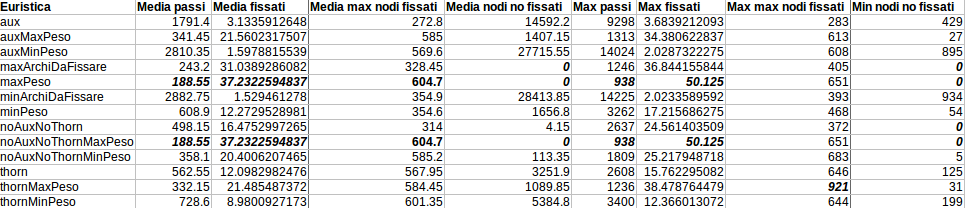
\includegraphics[width=\textwidth]{res/img/results.png}
\caption{Risultati delle euristiche sulle diverse metriche.}
\label{fig:results}
\end{figure}

La tabella mostra i risultati delle euristiche proposte sulle metriche presentate sopra. I migliori risultati per ogni metrica sono evidenziati in grassetto. 

Come si può vedere, l'euristica \textit{noAuxnoThornMaxPeso}, insieme all'euristica \textit{maxPeso}, sono quelle che, generalmente, portano ai migliori risultati. Non solo: i risultati di entrambe le euristiche sono gli stessi su ogni metrica. Questo significa che l'euristica \textit{maxPeso}, che favorisce i nodi a cui è assegnato peso maggiore, sembra essere la migliore per i problemi considerati, ma che prendere in considerazione la classe del nodo oltre al suo peso non porta alcuna variazione nei risultati.



%\begin{table}[H]
%\centering
%\caption{My caption}
%\label{my-label}
%\begin{tabular}{lllllllll}
%\textbf{Euristica}  & \textbf{Media passi}     & \textbf{Media fissati}          & \textbf{Media max nodi fissati} & \textbf{Media nodi no fissati} & \textbf{Max passi}    & \textbf{Max fissati}     & \textbf{Max max nodi fissati} & \textbf{Min nodi no fissati}             \\
%aux                 & 1791.4                   & 3.13359126475                   & 272.8                           & 14592.2                        & 9298                  & 3.68392120934            & 283                           & 429                                      \\
%auxMaxPeso          & 341.45                   & 21.5602317507                   & 585.0                           & 1407.15                        & 1313                  & 34.3806228374            & 613                           & 27                                       \\
%auxMinPeso          & 2810.35                  & 1.59788155387                   & 569.6                           & 27715.55                       & 14024                 & 2.02873222749            & 608                           & 895                                      \\ \cline{9-9} 
%maxArchiDaFissare   & 243.2                    & 31.0389286082                   & 328.45                          & \textit{\textbf{0.0}}          & 1246                  & 36.8441558442            & \multicolumn{1}{l|}{405}      & \multicolumn{1}{l|}{\textit{\textbf{0}}} \\ \cline{9-9} 
%maxPeso             & \textit{\textbf{188.55}} & \textit{\textbf{37.2322594837}} & \textit{\textbf{604.7}}         & \textit{\textbf{0.0}}          & \textit{\textbf{938}} & \textit{\textbf{50.125}} & 651                           & \textit{\textbf{0}}                      \\
%minArchiDaFissare   & 2882.75                  & 1.52946127802                   & 354.9                           & 28413.85                       & 14225                 & 2.0233589592             & 393                           & 934                                      \\
%minPeso             & 608.9                    & 12.2729528981                   & 354.6                           & 1656.8                         & 3262                  & 17.2156862745            & 468                           & 54                                       \\
%noAuxNoThorn        & 498.15                   & 16.4752997265                   & 314.0                           & 4.15                           & 2637                  & 24.5614035088            & 372                           & \textit{\textbf{0}}                      \\
%noAuxNoThornMaxPeso & \textit{\textbf{188.55}} & \textit{\textbf{37.2322594837}} & \textit{\textbf{604.7}}         & \textit{\textbf{0.0}}          & \textit{\textbf{938}} & \textit{\textbf{50.125}} & 651                           & \textit{\textbf{0}}                      \\
%noAuxNoThornMinPeso & 358.1                    & 20.4006207465                   & 585.2                           & 113.35                         & 1809                  & 25.2179487179            & 683                           & 5                                        \\
%thorn               & 562.55                   & 12.0982982476                   & 567.95                          & 3251.9                         & 2608                  & 15.762295082             & 646                           & 125                                      \\
%thornMaxPeso        & 332.15                   & 21.485487372                    & 584.45                          & 1089.85                        & 1236                  & 38.4787644788            & \textit{\textbf{921}}         & 31                                       \\
%thornMinPeso        & 728.6                    & 8.9800927173                    & 601.35                          & 5384.8                         & 3400                  & 12.3660130719            & 644                           & 199                                     
%\end{tabular}
%\end{table}